\chapter{Introduction to Radio Transients} \label{chap:introduction}
\pagenumbering{arabic}


\epigraph{\small\itshape “the Universe, she's whispering so softly I can hear, all the croaking insects, all the taxicabs, all the bum's spent change all the boys playing ball in the alleyways” \raggedleft\par--- \textup{ Gregory Alan Isakov, \textit{The Universe}}}

Throughout history humanity has watched the stars and observed transient phenomena. From prehistoric observers sat around campfires catching glimpses of comets and interpreting them as omens, to Chinese astronomers noting the Crab supernovae in 1054. The night sky has always captivated questions from how the Universe works to humanities place in it. Modern day astronomy at its core is the same, the awe still remains, but the tools have got sharper. With the advent of modern instrumentation the study of transients has expanded from the longest wavelength's to the highest energies.  As a result over the last century new classes of transients have emerged with their own sets of open questions. 

Transients include a large amount of objects that emit across the entire electromagnetic spectrum, it is generally used an umbrella term to include any astronomical objects that is time-dependent on times scales from nanoseconds to years. This thesis focuses on transients that emit radio waves $(\lambda \approx \text{mm}-\text{km})$.  
Radio waves can be emitted from an astrophysical object by either thermal or non-thermal emission. Any particle above 0~K vibrates when charged particles in atoms undergo acceleration they release electromagnetic radiation. As a consequence of this any particle above 0~K emits thermal radiation through two mechanisms blackbody or bremsstrahlung emission. Alternatively non-thermal emission arises from particles that have non-thermal motion also known as a non-Maxwellian energy distribution. These particles experience external forces that cause motion such as acceleration due to the presence of a magnetic field which commonly produce synchrotron radiation as relativistic electrons spiral around magnetic field lines. 

These emission mechanisms are observed across a wide range of astrophysical phenomena, from objects within Earth’s local neighbourhood such as solar flares, aurorae, and lightning in the outer planets, to some of the most distant and energetic known events including fast radio bursts and gamma-ray bursts. Radio transients span broad ranges of timescales, luminosity, and physical origin. In addition to observed sources, many theoretical radio transients have also been proposed but remain undetected, including primordial black holes, cosmic strings, and, more speculatively, technosignatures from extraterrestrial civilizations.

This chapter aims to non-exhaustively discuss the background and present motivation for studying natural and artificial transients. 

\section{Non-thermal Emission}

Electromagnetic emission can arise in plasmas from both bound atomic systems and unbound particles that are accelerated by external fields. Bound particles have quantized energies and the transition to lower energy states generates photons. However, unbound particles have a continuum of possible energies such that acceleration of these unbound particles can produce a continuum of photon energies. 

For a free (unbound), non-thermal and non-relativistic electron of charge, $e$ and mass $m_e$ that moves in a uniform magnetic field, $\mathbf{B} = \hat z B$. The only Lorentz force present is, $\mathbf{F} = -e(\mathbf{v} \times \textbf{B})$. If this electron is then placed in a circular orbit with a given speed, $v$ and a given radius $r$ the centipedal force causes an acceleration such that, 

\begin{equation}
    \frac{m_ev^2}{r} =evB
\end{equation}

Examining the angular frequency caused by the force balance, $\omega = v/r$. Substituting the following expression is obtained.

\begin{equation}
    \omega_L = \frac{eB}{m_ec} = 2.8~\frac{\text{B}}{\text{G}}~ \text{MHz}
    \label{eq: Larmor Freq}
\end{equation}

\Cref{eq: Larmor Freq} is known as the Larmor frequency, It's significant for setting the fundamental time and frequency scale for how charged particles can gyrate in a magnetic field. However, in an astrophysical context relativistic effects need to be accounted for where $\gamma>1$. With the same setup as before but now with a relativistic electron in a magnetic field, the Lorenz force in this case now takes the form of, 

\begin{equation}
    \frac{d p_\perp}{dt} = e \textbf{v}_\perp B
\end{equation}

Where $p_\perp$ is the transverse component of moment, $\textbf{p}_\perp = \gamma m_e \textbf{v}_\perp$. So relativistically the gyro-frequency of a particle is given by the following substitution, $\omega = \textbf{v}_\perp / r$ which results in, 

\begin{equation}
    \omega = \frac{eB}{\gamma m_ec}
    \label{eq:RealtivisticGyroFreq}
\end{equation}

\begin{figure}[t]
    \centering
    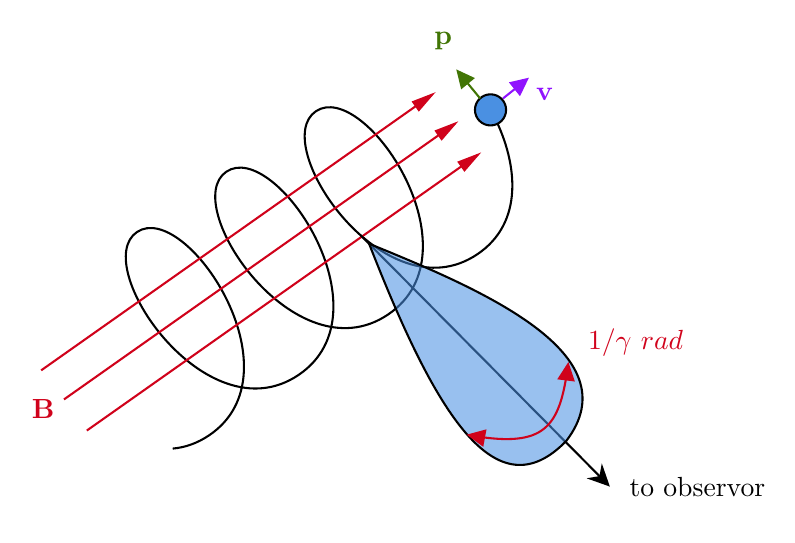
\begin{tikzpicture}[x=0.75pt,y=0.75pt,yscale=-1,xscale=1]
%uncomment if require: \path (0,441); %set diagram left start at 0, and has height of 44

%Shape: Spring [id:dp35001234639324486] 
\draw   (326.33,156.84) .. controls (337.71,179.51) and (340.59,207.91) .. (318.21,223.02) .. controls (273.46,253.23) and (217.16,169.83) .. (240.36,154.16) .. controls (263.57,138.5) and (319.87,221.9) .. (275.11,252.11) .. controls (230.36,282.32) and (174.06,198.92) .. (197.26,183.26) .. controls (220.47,167.59) and (276.77,250.99) .. (232.01,281.21) .. controls (187.26,311.42) and (130.96,228.01) .. (154.17,212.35) .. controls (177.37,196.68) and (233.67,280.09) .. (188.91,310.3) .. controls (183.19,314.16) and (177.28,316.17) .. (171.37,316.69) ;
%Shape: Circle [id:dp033919684441355846] 
\draw  [fill={rgb, 255:red, 74; green, 144; blue, 226 }  ,fill opacity=1 ] (317,153.5) .. controls (317,149.36) and (320.36,146) .. (324.5,146) .. controls (328.64,146) and (332,149.36) .. (332,153.5) .. controls (332,157.64) and (328.64,161) .. (324.5,161) .. controls (320.36,161) and (317,157.64) .. (317,153.5) -- cycle ;
%Straight Lines [id:da8239992919484788] 
\draw [color={rgb, 255:red, 208; green, 2; blue, 27 }  ,draw opacity=1 ]   (108,279) -- (128.62,264.46) -- (296.37,146.15) ;
\draw [shift={(298,145)}, rotate = 144.81] [fill={rgb, 255:red, 208; green, 2; blue, 27 }  ,fill opacity=1 ][line width=0.08]  [draw opacity=0] (12,-3) -- (0,0) -- (12,3) -- cycle    ;
%Straight Lines [id:da8706605995386824] 
\draw [color={rgb, 255:red, 208; green, 2; blue, 27 }  ,draw opacity=1 ]   (119,293) -- (139.62,278.46) -- (307.37,160.15) ;
\draw [shift={(309,159)}, rotate = 144.81] [fill={rgb, 255:red, 208; green, 2; blue, 27 }  ,fill opacity=1 ][line width=0.08]  [draw opacity=0] (12,-3) -- (0,0) -- (12,3) -- cycle    ;
%Straight Lines [id:da6748288379378818] 
\draw [color={rgb, 255:red, 208; green, 2; blue, 27 }  ,draw opacity=1 ]   (130,308) -- (150.62,293.46) -- (318.37,175.15) ;
\draw [shift={(320,174)}, rotate = 144.81] [fill={rgb, 255:red, 208; green, 2; blue, 27 }  ,fill opacity=1 ][line width=0.08]  [draw opacity=0] (12,-3) -- (0,0) -- (12,3) -- cycle    ;
%Straight Lines [id:da6673811504605812] 
\draw [color={rgb, 255:red, 65; green, 117; blue, 5 }  ,draw opacity=1 ]   (319.5,148) -- (309.9,136.32) ;
\draw [shift={(308,134)}, rotate = 50.6] [fill={rgb, 255:red, 65; green, 117; blue, 5 }  ,fill opacity=1 ][line width=0.08]  [draw opacity=0] (8.93,-4.29) -- (0,0) -- (8.93,4.29) -- cycle    ;
%Straight Lines [id:da10409690559320883] 
\draw [color={rgb, 255:red, 144; green, 19; blue, 254 }  ,draw opacity=1 ]   (330.5,148) -- (340.66,139.87) ;
\draw [shift={(343,138)}, rotate = 141.34] [fill={rgb, 255:red, 144; green, 19; blue, 254 }  ,fill opacity=1 ][line width=0.08]  [draw opacity=0] (8.93,-4.29) -- (0,0) -- (8.93,4.29) -- cycle    ;
%Straight Lines [id:da9875636651936046] 
\draw    (262,214) -- (379.89,332.87) ;
\draw [shift={(382,335)}, rotate = 225.24] [fill={rgb, 255:red, 0; green, 0; blue, 0 }  ][line width=0.08]  [draw opacity=0] (10.72,-5.15) -- (0,0) -- (10.72,5.15) -- (7.12,0) -- cycle    ;
%Curve Lines [id:da060929441107962834] 
\draw [fill={rgb, 255:red, 74; green, 144; blue, 226 }  ,fill opacity=0.57 ]   (266,218) .. controls (298,300) and (327,348) .. (361,313) ;
%Curve Lines [id:da15485160304368528] 
\draw [fill={rgb, 255:red, 74; green, 144; blue, 226 }  ,fill opacity=0.56 ]   (266,218) .. controls (320,240) and (393,271) .. (361,313) ;
%Curve Lines [id:da9741350174449808] 
\draw [color={rgb, 255:red, 208; green, 2; blue, 27 }  ,draw opacity=1 ]   (316.34,310.58) .. controls (350.36,316.21) and (357.69,306.65) .. (361.64,277.74) ;
\draw [shift={(362,275)}, rotate = 97.13] [fill={rgb, 255:red, 208; green, 2; blue, 27 }  ,fill opacity=1 ][line width=0.08]  [draw opacity=0] (8.93,-4.29) -- (0,0) -- (8.93,4.29) -- cycle    ;
\draw [shift={(313,310)}, rotate = 10.44] [fill={rgb, 255:red, 208; green, 2; blue, 27 }  ,fill opacity=1 ][line width=0.08]  [draw opacity=0] (8.93,-4.29) -- (0,0) -- (8.93,4.29) -- cycle    ;

% Text Node
\draw (345,141.4) node [anchor=north west][inner sep=0.75pt]  [color={rgb, 255:red, 144; green, 19; blue, 254 }  ,opacity=1 ]  {$\mathbf{v}$};
% Text Node
\draw (296,114.4) node [anchor=north west][inner sep=0.75pt]  [color={rgb, 255:red, 65; green, 117; blue, 5 }  ,opacity=1 ]  {$\mathbf{p}$};
% Text Node
\draw (370,257.4) node [anchor=north west][inner sep=0.75pt]    {$\textcolor[rgb]{0.82,0.01,0.11}{1/\gamma \ \text{rad}}$};
% Text Node
\draw (102,291.4) node [anchor=north west][inner sep=0.75pt]  [color={rgb, 255:red, 208; green, 2; blue, 27 }  ,opacity=1 ]  {$\mathbf{B}$};
% Text Node
\draw (390,329) node [anchor=north west][inner sep=0.75pt]   [align=left] {to observor};


\end{tikzpicture}
    \caption{Example of a relativistic electron in a magnetic field producing synchrotron radiation.}
    \label{fig:SyncotronicEmissionDiagram}
\end{figure}
\tikzset{every picture/.style={line width=0.75pt}} %set default line width to 0.75pt    


\Cref{eq:RealtivisticGyroFreq} sets the basic orbital timescale for synchrotron-emitting electrons. As the electron becomes relativistic $(\gamma>1)$ the electromagnetic waves are concentrated in a narrow cone of half-angle $\sim1/\gamma$ about the instantaneous velocity vector, $\textbf{v}$, towards the observer which is shown in \cref{fig:SyncotronicEmissionDiagram}.
Or in simpler terms in the electron's rest frame it will just gyrate in a circle at a frequency, $\omega_L$ and be a smooth sinusoid at that frequency. Whereas in the observer's frame, once the electron is relativistic it will be `squashed' due to aberration on a very narrow radiation cone of width, $\sim1/\gamma$ as stated above. The consequence of this is there will only be a single pulse per orbit as a very small fraction of the orbit is pointing towards the observer. For each of these short pulses there will be a spike in electric field as a function of time, with a pulse duration of $\Delta t \sim 1/\gamma^3 \cdot P_{e,\text{orb}}$. The spectrum of radiation of the short pulses is the Fourier transform of the pulse once time and aberration are taken into account. When a short pulse is Fourier transformed it will have power at many frequencies, forming a broad spectrum. So the characteristic frequency of the spectrum is $w_c \sim 1/\Delta t \sim \gamma^3 \omega_L$. This broad spectrum peaks near $\omega_c$, when this is integrated over a power-law distribution of electrons it produces a power-law synchrotron continuum which is observed in many radio transients. 
Pulsar, fast radio bursts, flare stars and long period transients are all examples of non-thermal radio sources. All of which emit coherent radio waves except flare stars which is discussed later in this chapter.

\subsection{The Transient Phase Space}

The transient phase space (shown in \cref{fig:phase_space:chap1}) was first coined by \cite{cordes_dynamic_2004} and is commonly used as a way to illustrate key characteristics of transient radio emission across known radio transients. The plot represents the observed frequency and emission duration (width) along with the spectral luminosity of the object. It also delineates the radio transient populations that exhibit coherent and incoherent emission. Here the lines represent minimum brightness temperature. This representation is an optimal way to quantify the science case for given telescope specifications. One thing that is important to note with this representation is that each point represents the centre of a distribution of emission, in reality there will be an array of luminosity and widths for repeating sources. 

\begin{figure}
    \centering
    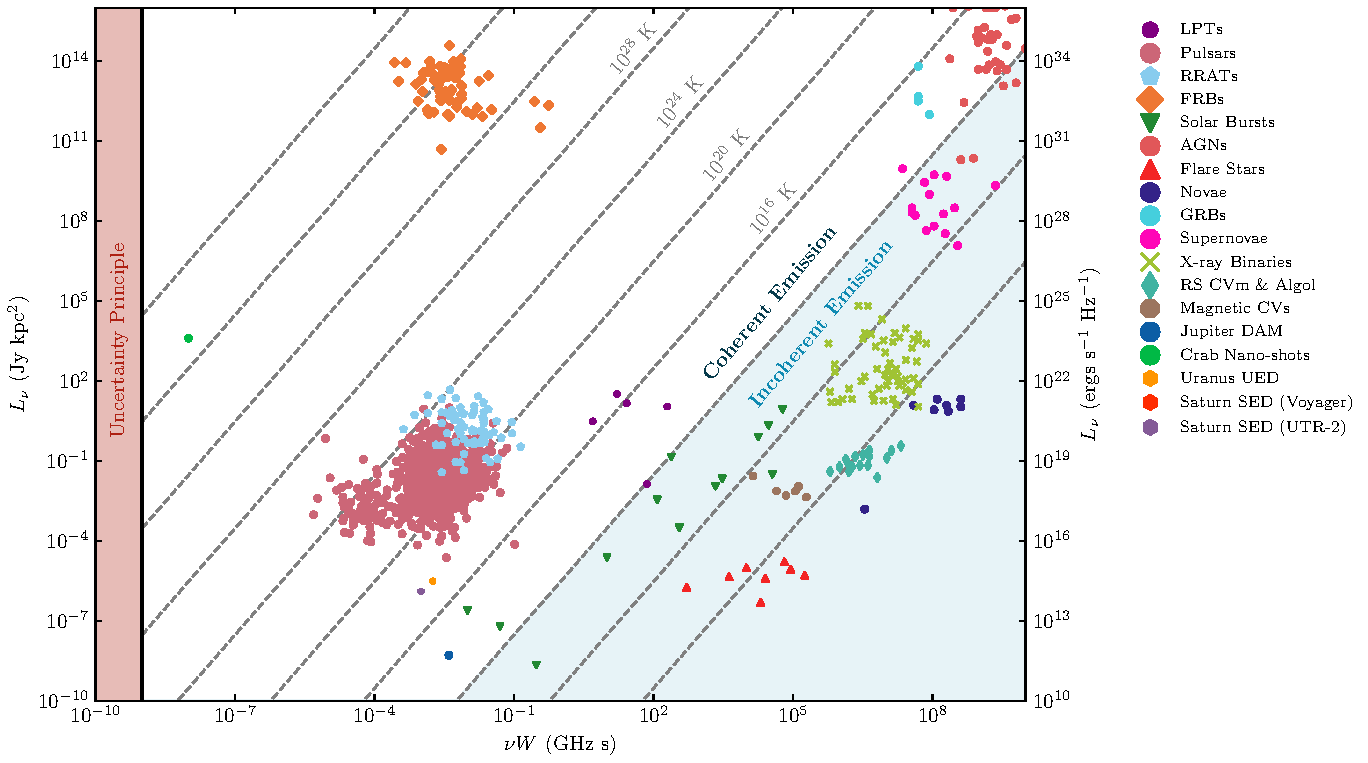
\includegraphics[width=0.9\linewidth]{chapter1/figures/phase_space.pdf}
    \caption{Transient Phase Space adapted from \citet[p. 24,][]{keane_thesis} showing a $\nu \text{W}$ vs. $L_\nu$. Where $\nu \text{W}$ represents the product of observed frequency and pulse width and $L_\nu$ shows the spectral luminosity. Data collected by }
    \label{fig:phase_space:chap1}
\end{figure}

This thesis focuses on transient searching, with a more specific focus on pulsars and technosignatures, however a large portion of this work is based in the finding transients at low frequencies. The rest of this chapter will discuss the theoretical background and literature for an array of radio transients, with the detail of each reflective of the novel work that is present. 

\section{Neutron Stars and Pulsars}

\subsection{A Prelude to Pulsars}

When stars with a mass of at least $8 \smass$ reach the end of their evolutionary stage they experience a depletion of nuclear fuel will and undergo a core collapse.  This results in the star exploding as a supernova. Depending on the mass of the host star the Supernova will form a black Hole or a neutron Star. Based on the electron degeneracy pressure limit \citep[pp. 434 -- 443]{chandrasekhar_introduction_2012} stars that fall in the range of 20 - 30 $\smass$ form neutron stars \citep{heger_how_2003}. \

Neutron stars are supported against further collapse by the presence of neutron degeneracy pressure which arises from the Pauli exclusion principle. Strong nuclear forces between the neutrons also provides additional support against gravitational collapse. With these three opposing forces a stable equilibrium is formed \citep{1983bhwd.book.....S}. \

In turn, this makes neutron stars exceptionally dense, they are the densest known objects in the universe that emit light. The average density of a neutron star is $10^{17} \text{kg/m}^3$ \citep{baym_neutron_1971} and their radii are comparable to the size of cities, with radii of 10--20 km. \

During collapse the conservation of magnetic flux plays a crucial role in the large strength magnetic fields that are observed in neutron stars along with contributions from the dynamo effect and frozen-in magnetic fields. The strength of a pulsar's magnetic field is on the order of $10^{12}$ - $10^{15}$ G \citep{michel_theory_1982}. \

Charged particles accelerate along the magnetic field lines in the magnetosphere of the neutron star. These particles emit electromagnetic radiation in a cone shape along the magnetic axis. If the magnetic axis is not aligned with the rotational axis of the neutron star, the radiation beam will sweep across the sky. This is known as a pulsar, a Galactic lighthouse.% analogus to cosmic lighthouses. 

\begin{figure}[t]
    \centering
    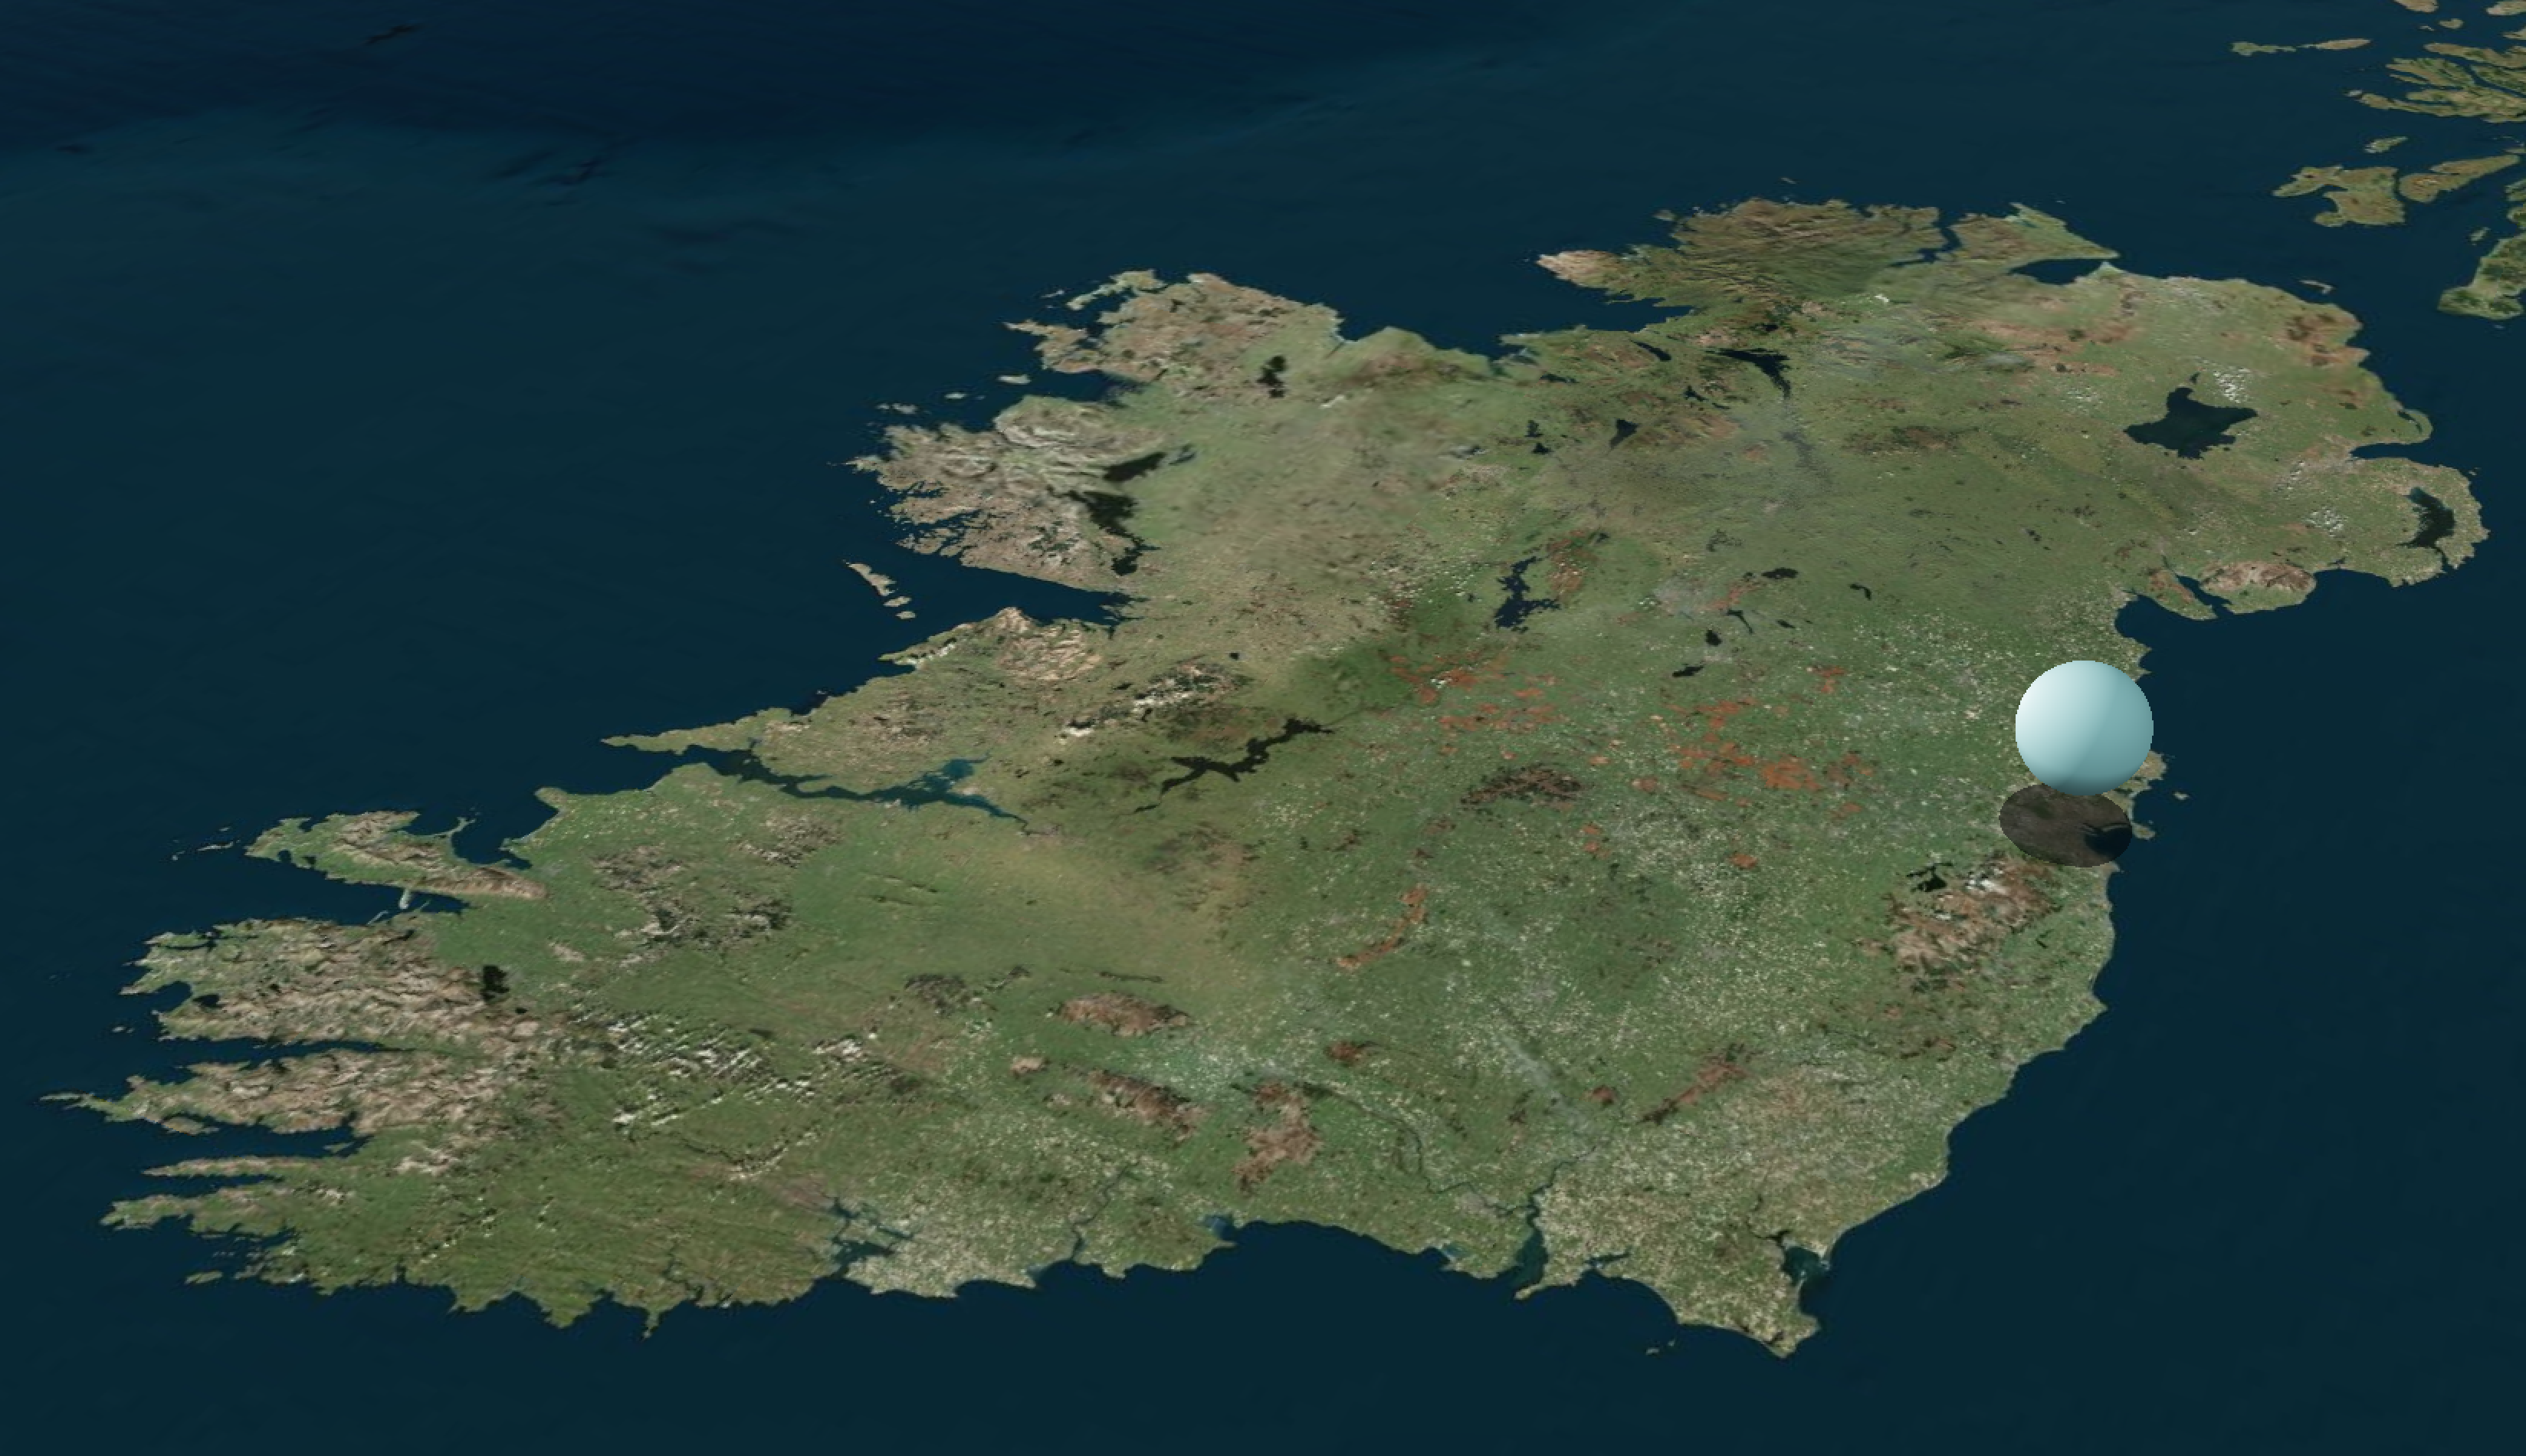
\includegraphics[width=0.8\linewidth]{chapter1/figures/ns-dublin.png}
    \caption{A canonical pulsar of $1.4 \smass$ positioned above House 1, Trinity College Dublin. Courtesy of Daniel Wysocki and HanGyeol Suh}
    \label{fig:placeholder}
\end{figure}


\subsection{The Population of Pulsars}

At the time of writing, there are currently more than 3380 known pulsars. Since their discovery by Jocelyn Bell Burnell \citep{hewish_observation_1968}, the population has grown immensely, but there remain many open questions about pulsar evolution and the subclasses that lie within the population as a whole. Similarly to how exoplanet populations are shown using the mass-radius diagram and stellar populations are shown using the Hertzsprung-Russell diagram, pulsar populations are shown using what is known as the $P-\dot P$ diagram.

$P$ represents the pulsar's rotational period and $\dot P$ its derivative. These are key ways that pulsars are classified and studied in the context of their evolution. An example of a $P-\dot P$ diagram is shown in \cref{fig:p-pdot}. Different values on the plot indicate roughly the pulsar's age and magnetic field strength. \Cref{fig:p-pdot} shows the vastly different values between pulsars in the millisecond range and pulsars in the second range.

Theoretically, it has been shown that pulsars can be related to a ``death" line in the $P-\dot P$ diagram. This is the line where pulsars are no longer able to emit radio waves due to the pulsar's magnetic field no longer being strong enough to accelerate particles along the magnetic field lines. However, it has been shown that pulsars do exist below this line. The area below this line is commonly referred to as the ``graveyard".

\begin{figure}
    \centering
    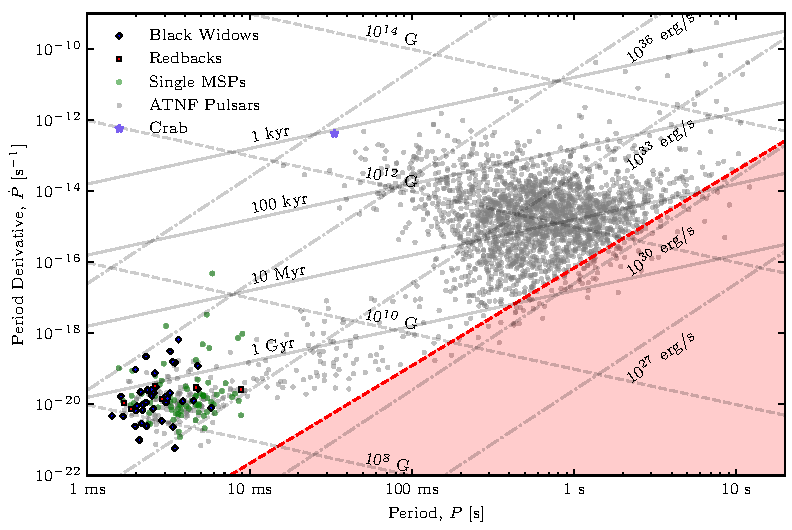
\includegraphics[width=0.8\textwidth]{chapter1/figures/PPdot-diagram.pdf}
    \caption{The $P-\dot P$ diagram showing the population of pulsars. The millisecond pulsar subclasses are colour coded. The red region represents the death line, where pulsars are theoretically no longer able to emit radio waves.}
    \label{fig:p-pdot}
\end{figure}

\subsection{The Properties of Pulsars}

The following section gives a brief non-exhaustive overview of some of the key properties of pulsars. 

\subsubsection{Neutron Star Radius \& Mass}

Understanding the mass of pulsars is important for understanding their evolution and equation of state. \cite{oppenheimer_massive_1939} derived a canonical mass limit of neutron stars to be 1.4 $\mathrm{M_{\odot}}$, but experimentally, this has been shown to be higher, with the largest mass of a pulsar observed to be $\sim 2.35 \mathrm{M_{\odot}}$ \citep{Romani_2022}. The mass-radius relationship of a pulsar is defined by an equation of state and a maximum mass limit. Redshifts and gravitational effects observed in pulsars exhibit the observed temperature and flux to be smaller than the actual value. The observed radius $R_\text{obs}$ can be described as follows \citep[p. 56][]{pulsar_handbook}:

\begin{equation}
    R_\text{obs} = \frac{R}{\sqrt{1 - \frac{2GM}{Rc^2}}} = \frac{R}{ \sqrt{1 - \dfrac{R_s}{R}}}
\end{equation}

where $R$ is the pulsar's radius and $M$ is the gravitational mass, $G$ is the gravitational constant, $c$ is the speed of light and $R_s$ is the Schwarzschild radius. \
The lower limit of the neutron star radius is described by \cite[p. 58][]{pulsar_handbook}: 

\begin{equation}
    R_\text{min} \simeq 1.5 \ R_s = \frac{3GM}{c^2} = 6.2 \ \text{km.} \left( \frac{M}{1.4 \smass} \right)
\end{equation}

Opposite to this the upper limit of the radius is obtained by requiring that there is stability against breaking up due to centrifugal forces. This gives \cref{eq:radius-max} following as described in \cite[p.~58]{pulsar_handbook}. 

\begin{equation}
    R_\text{max} \simeq \left(\frac{GMP^2}{4 \pi^2}\right)^{1/3} = 16.8 \ \text{km} \left( \frac{M}{1.4 \smass} \right)^{1/3} \left( \frac{P}{\text{ms}} \right)^{2/3}
    \label{eq:radius-max}
\end{equation}

Most pulsars are theoretically thought to have radii in the range of 10–15 km \citep{lattimer_neutron_2001}, giving them the unique position of `almost' black holes. 

\subsubsection{Spin Evolution}
One of the unique characteristics of pulsars is the spinning that they exhibit. Understanding the spin evolution gives insight into many parameters of the pulsars, most notably the stage of their evolution. Pulsars begin their life in the upper end of the $P-\dot P$ diagram and slowly move down and to the right as they age due to a loss in rotational energy, commonly referred to as spin-down luminosity. The spin-down ($\dot E$) is described as follows \citep[p.~59]{pulsar_handbook}:

\begin{equation}
\dot E = - \frac{dE_{\text{rot}}}{dt} = 4\pi^2 I \dot P P^{-3}
\label{eq:spin-down-energy}
\end{equation}

Where $I$ is the moment of inertia. It is important to note that the energy loss that is converted into radio emission is almost negligible in comparison to the total energy loss from spin down. 

% \subsubsection{Radio Emission Beam}

% Pulse width

% \begin{equation}
%     \cos \rho = \cos \alpha \cos (\alpha + \beta) + \sin \alpha \sin (\alpha + \beta) \cos \left( \frac{W}{2} \right)
% \end{equation}

\subsubsection{Braking Index}

Pulsars have strong magnetic dipoles. According to classical mechanics, a rotating magnetic dipole that exhibits a moment, $|m|$, emits an electromagnetic wave at the pulsar's rotation frequency \citep[p.~60]{pulsar_handbook}. The dipole's radiation power is characterized by:

\begin{equation}
    \dot E_{\text{dipole}} = \frac{2}{3c^3} |m|^2 \omega^4 \sin^2 \alpha
\end{equation}

Where $\alpha$ is the angle between the magnetic axis and the rotation axis. Equating the above equation to the loss of rotational energy described in \cref{eq:spin-down-energy} gives the following for the expected evolution of the period:

\begin{equation}
    \dot \Omega = - \frac{2}{3Ic^3} |m|^2 \Omega^3 \sin^2 \alpha
\end{equation}

This is more commonly written as a power law, 

\begin{equation}
    \dot \nu = -K \nu^n 
    \label{eq:spin-down-power-law}
\end{equation}

\Cref{eq:spin-down-power-law} in terms of the period is $\dot P = K P^{2-n}$. Since this is a first-order differential equation, the solution can be integrated and given a constant, $K$, which provides an expression of age:

\begin{equation}
    T = \frac{P}{(n-1)\dot P} \left\{ 1 - \left( \frac{P_0}{P} \right)^{n - 1} \right\} 
    \label{eq:age-full}
\end{equation}

Here $P_0$ is the initial period of the pulsar. Commonly an assumption is made that the current period is much greater than the initial period $(P_0 \ll P)$. If it is also assumed that the pulsar is spinning down to due dipole magnetic radiation ($n=3$), \cref{eq:age-full} can be simplified into a characteristic age. 

\begin{equation}
    \tau_c \cong 15.8~\text{Myr} \left( \frac{P}{s} \right) \left( \frac{\dot P}{10^{-15}} \right)^{-1}
\end{equation}

The above estimation for a pulsars age is known to be inconsistent with theory to varying degrees. In cases where Supernovae has been observed and has produced a pulsar the age is known to a much higher degree of accuracy. The Crab pulsar is one such example with an observed Supernova event in 1054 AD by Chinese astronomers \citep{kaspi_chandra_2001}. %Supernoave remnants are also used to estimate the age of pulsars. 

\subsubsection{Dispersion Measure} \label{sec:DispersionMeasure}

The interstellar medium (ISM) is a complex mixture of gas, dust and magnetic fields that fills the space between stars in a galaxy. Given that the ISM is a cold and ionised plasma any electromagnetic radiation will undergo a frequency-dependant index of refraction as they propagate. The following equation describes the refractive index of the ISM neglecting Galactic magnetic field \citep[p.~85]{pulsar_handbook},

\begin{equation}
    \mu = \sqrt{1 - \left( \frac{f_p}{f} \right)^2}
    \label{eq: ism-refractive-index}
\end{equation}

Where $f_p$ is the plasma frequency, $8.5 ~\text{kHz} \left(n_e/\text{cm}^{-3} \right)^{1/2}$ and $f$ is the frequency of the observed radiation. \\ If the refractive index of the ISM $\mu < 1$ then it can be assumed that the group velocity of the radiation is $v_g = c\mu$ which is sub light speed. The path of radiation from a pulsar to the observer will be delayed in time with respect to an infinite frequency by an amount:

\begin{equation}
    t = \left( \int^d_0 \frac{dl}{v_g} \right) - \frac{d}{c}
\end{equation}

If is assumed to be $f_p \ll f$, $\mu$ can be approximated.

\begin{equation}
    t = \frac{1}{c} \int^d_0 \left(1 + \frac{f_p^2}{2f^2} \right) dl - \frac{d}{c}  = \frac{e^2}{2 \pi m_e c} \dfrac{\int^d_0 n_e ~dl}{f^2} \equiv \mathcal{D} \cdot \dfrac{\text{DM}}{f^2}
\end{equation}

Where $\mathcal{D}$ is the dispersion constant and $\text{DM}$ is the dispersion measure. Each are commonly expressed as follows, $\mathcal{D}= 4.15 \times 10^3 ~\text{MHz}^2 ~\text{pc}^{-1} ~ \text{cm}^3 ~\text{s}$ and $\text{DM} = \int^d_0 n_e ~dl ~\text{cm}^{-3} ~\text{pc}$. This definition was adapted from \citet[p.~86]{pulsar_handbook} and \cite{taylor_recent_1977}.

\section{Other Radio Transients and where to find them}

\subsection{Fast Radio Bursts}

\subsection{Long Period Transients}

\subsection{Radio Flare Stars}

% \subsection{Gamma Ray Bursts} % Maybe chuck in the misc chapter. 

\section{The Search for Intelligent Life in the Universe}

Arguably one of the most captivating and difficult problems in astronomy is on the question of life elsewhere in the Universe. It's a problem where the known population is statistical insignificant given that Earth is the only known example. However, in the last 50 years evidence has steadily mounted that the conditions for life in the universe are relativity common. Since exoplanets were first directly detected in 1992 there is (at the time of writing) over 6,300 confirmed exoplanets of all varieties \citep{NEA12}. It is also a popular opinion that most of the stars within the Galaxy and by extent the Universe have orbiting planets. % Even if a minute amount of planets give rise to life there should be 

However, postulating the conditions in which life evolves and lives long enough and becomes advanced enough for interstellar communications is highly difficult and highly speculative. The search for extraterrestrial intelligence (SETI) has likely been around for 100's of years. But early formal discussions arose in the 19th and 20th centuries, specifically around Mars. Nikola Tesla thought about communication with Martians using a wireless electrical system, Giovanni Schiaparelli argued the case for canals on Mars. 

The birth of modern SETI is generally attributed with \cite{CocconiMorrison1959}'s seminal paper on interplanetary radio communication, around 7 months later Project Ozma was carried out by \cite{Drake:1961bv}. Drake used the 85 ft telescope at the Green Bank Observatory (GBO) to search two nearby stars Tau Ceti and Epsilon Eridani for civilizations broadcasting in radio. Following this Drake hosted a meeting to discuss paths forward for the field, in preparing for the meeting Drake coined an equation to estimate the prevalence of life in the Milky Way, 

\begin{equation}
    \boxed{
    N = R_* f_p N_e f_l f_i f_c L 
    }
    \label{eq:Drake_equation}
\end{equation}


 In this expression $N$ is the number of communicative civilizations in the Milky Way galaxy, $R_{*}$ is the rate of star formation per year in the galaxy, $f_{p}$ is the fraction of stars that have planets around them, $n_{e}$ is the average number of planets that can potentially support life per star that has planets, $f_{l}$ is the fraction of potentially life-supporting planets that actually develop life, $f_{i}$ is the fraction of planets with life that go on to develop intelligent life and $f_{c}$ is the fraction of civilizations that develop a technology that releases detectable signs of their existence into space. \Cref{eq:Drake_equation} is meant more as a thought experiment, rather than an explicit and empirical value as most the values in the equations have debatable definitions and constraints, especially the last 3 factors. Asking members of the radio transient group, based purely on intuition given somewhat known limits for the first two terms yield answers from 0 to 761. The 0 answer includes Earth, alluding that many consider the definition of intelligence to be something outside the current conventional definition\footnote{\url{https://dictionary.apa.org/intelligence}}. Frank Drake's number plate read NEQLSL, which estimated that the number of civilizations in the Galaxy was determined by their ability to have prolonged lifetimes. 

 Since the inception of the Drake equation and Project Ozma there has been an increasing effort throughout the decades to conduct SETI\footnote{For a comprehensive history see X}. 

\subsection{Artificial Radio Transients}

\subsection{Breakthrough Listen}

